\documentclass[handout,nooutcomes]{ximera}
\usepackage{booktabs}
%% handout
%% space
%% newpage
%% numbers
%% nooutcomes

\renewcommand{\outcome}[1]{\marginpar{\null\vspace{2ex}\scriptsize\framebox{\parbox{0.75in}{\begin{raggedright}P\arabic{problem} Outcome: #1\end{raggedright}}}}}

\renewenvironment{freeResponse}{
\ifhandout\setbox0\vbox\bgroup\else
\begin{trivlist}\item[\hskip \labelsep\bfseries Solution:\hspace{2ex}]
\fi}
{\ifhandout\egroup\else
\end{trivlist}
\fi}

\newcommand{\RR}{\mathbb R}
\renewcommand{\d}{\,d}
\newcommand{\dd}[2][]{\frac{d #1}{d #2}}
\renewcommand{\l}{\ell}
\newcommand{\ddx}{\frac{d}{dx}}
\everymath{\displaystyle}
\newcommand{\dfn}{\textbf}
\newcommand{\eval}[1]{\bigg[ #1 \bigg]}


\title{Breakout Session 14: Related Rates (Part I)}

\begin{document}
\begin{abstract}
  \textbf{A look back:} In the previous (February 23, 2016) Breakout Session you practiced differentiating inverse functions.

  \textbf{Overview:} In today's (February 25, 2016) Breakout Session you'll be introduced to an important application of derivatives: related rates.
  
  \textbf{A look ahead:} In the next (March 1, 2016) Breakout Session you continue to practice related rates and learn another important application of derivatives: locating local extrema.
\end{abstract}
\maketitle

\section{Learning Outcomes}
\label{section:learning-outcomes}
The following outcomes are \emph{not an exhaustive} list of the skills you will need to develop and integrate for demonstration on quizzes and exams.
This list is meant to be a starting point for conversation (with your Lecturer, Breakout Session Instructor, and fellow learners) for organizing your knowledge and monitoring the development of your skills.

\begin{itemize}
  \item 
    Identify word problems as related rates problems.
  \item 
    Translate word problems into mathematical expressions.
  \item 
    Calculate derivatives of expressions with multiple variables implicitly.
  \item 
    Understand the process of solving related rates problems.
  \item
    Solve related rates word problems.
\end{itemize}
\newpage

\begin{image}
 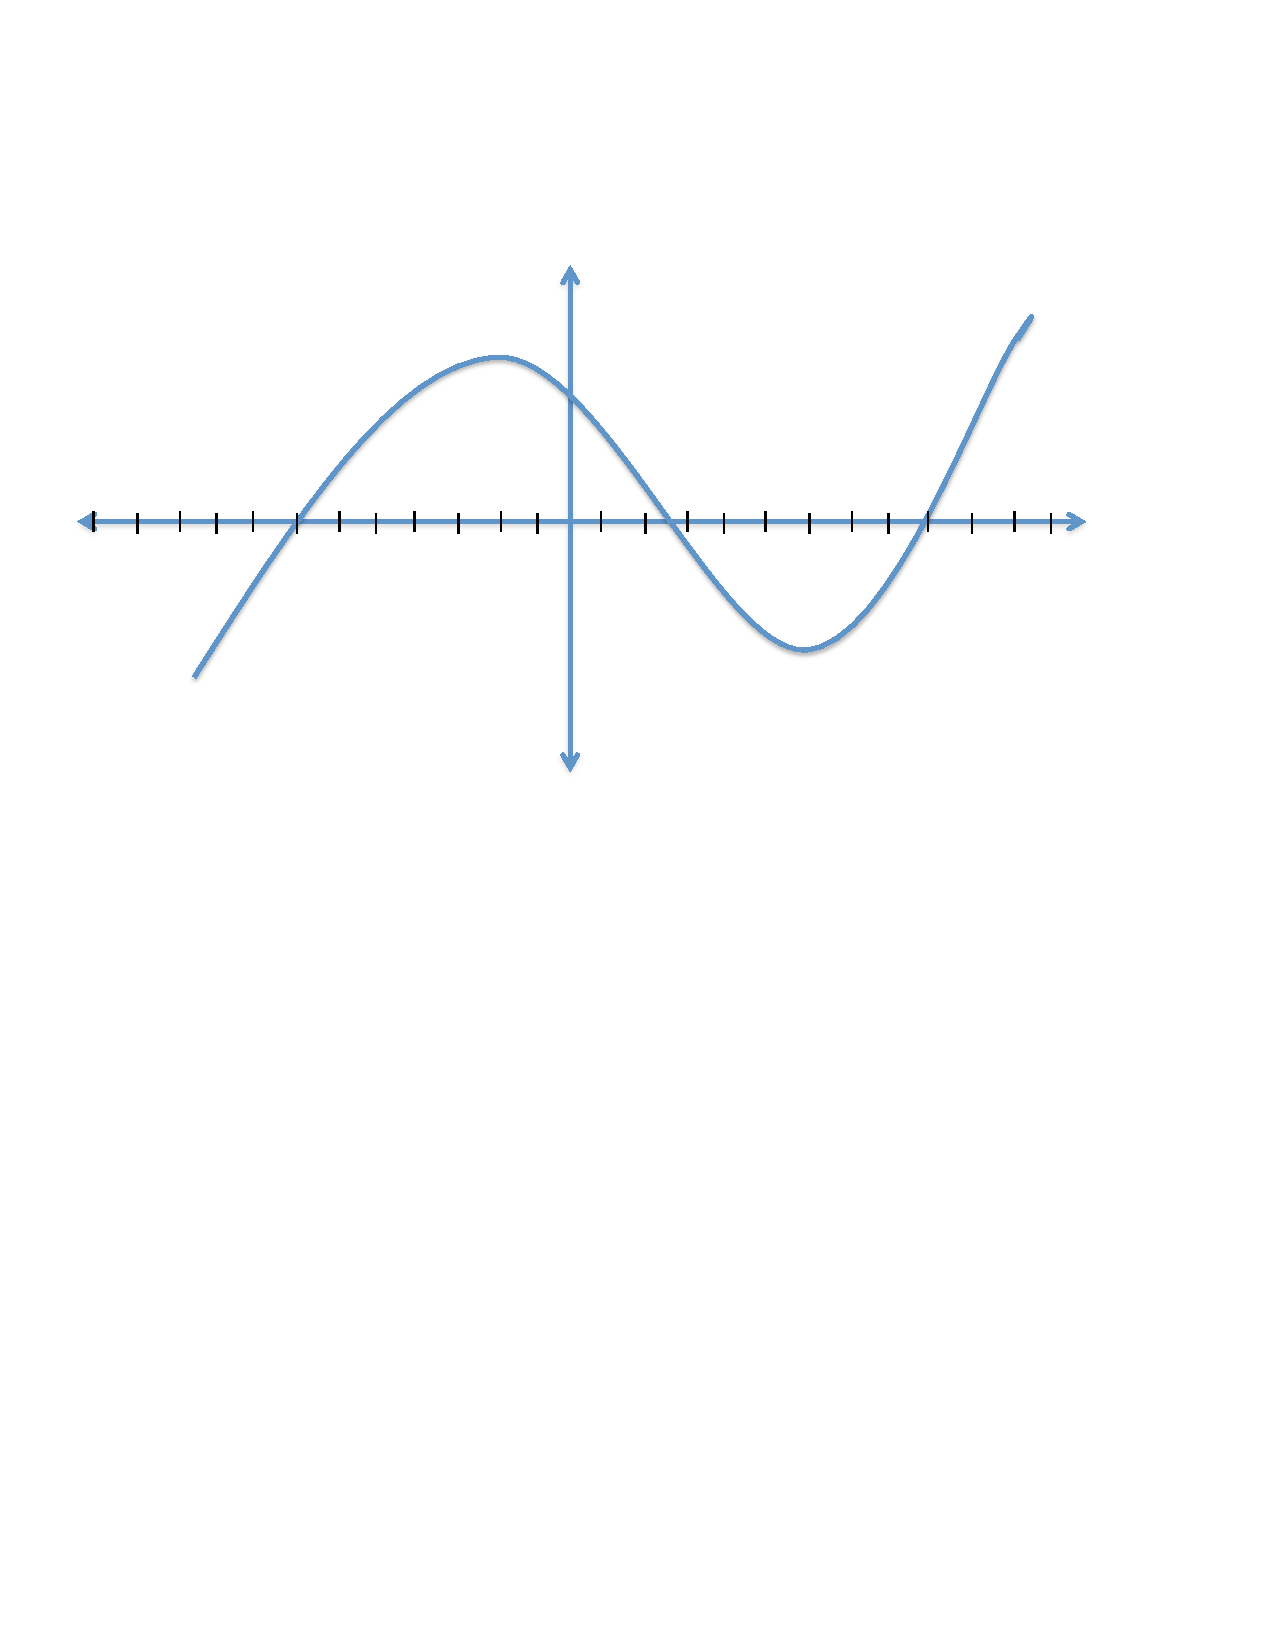
\includegraphics[trim= 220 480 250 90]{Images/Figure2.pdf}
\end{image}


\begin{problem}
  A hot air balloon is 150 ft above the ground when a motorcycle passes directly beneath it traveling at a rate of 60 ft/sec (in a straight line on a horizontal road).
  If the balloon is rising vertically at a rate of 10 ft/s, what is the rate of change of the distance between the motorcycle and the balloon 10 seconds later?
  \begin{freeResponse}
    Let $P$ denote the point on the ground directly below the hot air balloon, let $x$ denote the distance from the motorcycle to $P$, let $y$ denote the distance from the hot air balloon to $P$, and let $z$ denote the distance from the motorcycle to the hot air balloon.
    The location of the motorcycle, the hot air balloon, and the point $P$ form a right triangle, and so we have that
    \begin{equation}\label{Pythagorean}
      x^2 + y^2 = z^2.
    \end{equation}
    We are given that $\dd[x]{t} = 60$ and $\dd[y]{t} = 10$, and the question asks us to find $\dd[z]{t}$ at time $t=10$ (meaning 10 seconds after the motorcycle passes the point $P$).
    We can also easily compute that:
		$$ x(10) = 60 \cdot 10 = 600 ft $$
		$$ y(10) = 150 + (10 \cdot 10) = 250 ft $$
		$$ z(10) = \sqrt{ 600^2 + 250^2} = \sqrt{360000 + 62500} = \sqrt{422500} = 650 ft $$
		where $x(10), y(10), and $z(10) denote the values of $x$, $y$, and $z$ 10 seconds after the motorcycle passes the point $P$.  
		
                Differentiating equation \ref{Pythagorean} with respect to time, substituting, and solving for $\dd[z]{t}$ yields:
		$$ 2x \dd[x]{t} + 2y \dd[y]{t} = 2z \dd[z]{t} $$
		$$ x \dd[x]{t} + y \dd[y]{t} = z \dd[z]{t} $$
		$$ (600)(60) + (250)(10) = (650) \dd[z]{t} $$
		$$ \dd[z]{t} = \frac{36000 + 2500}{650} \frac{ft}{sec} = \frac{3850}{65} \frac{ft}{sec} = \frac{770}{13} \frac{ft}{sec} \approx 59.23 \frac{ft}{sec} $$
		\end{freeResponse}
\end{problem}

\begin{problem}
  The bottom of a 7 ft ladder, leaning against a (vertical) wall, is sliding away from the wall at a constant rate.
  Is the top of the ladder falling down at a constant rate too?
  Why or why not?
\end{problem}

\section{Extra Problem for Personal Practice}
\begin{problem}
  Find the mistake in the solution to the given problem:

  \begin{quote}
    Two boats leave from the same dock, but at slightly different
    times.  One boat is traveling east at 30mph while the other boat
    is traveling north at 15mph.  At an instant in time when the boat
    traveling east is 15 miles from the dock and the boat traveling
    north is 10 miles away from the dock, what rate is the distance
    between the boats changing?
    \begin{image}
      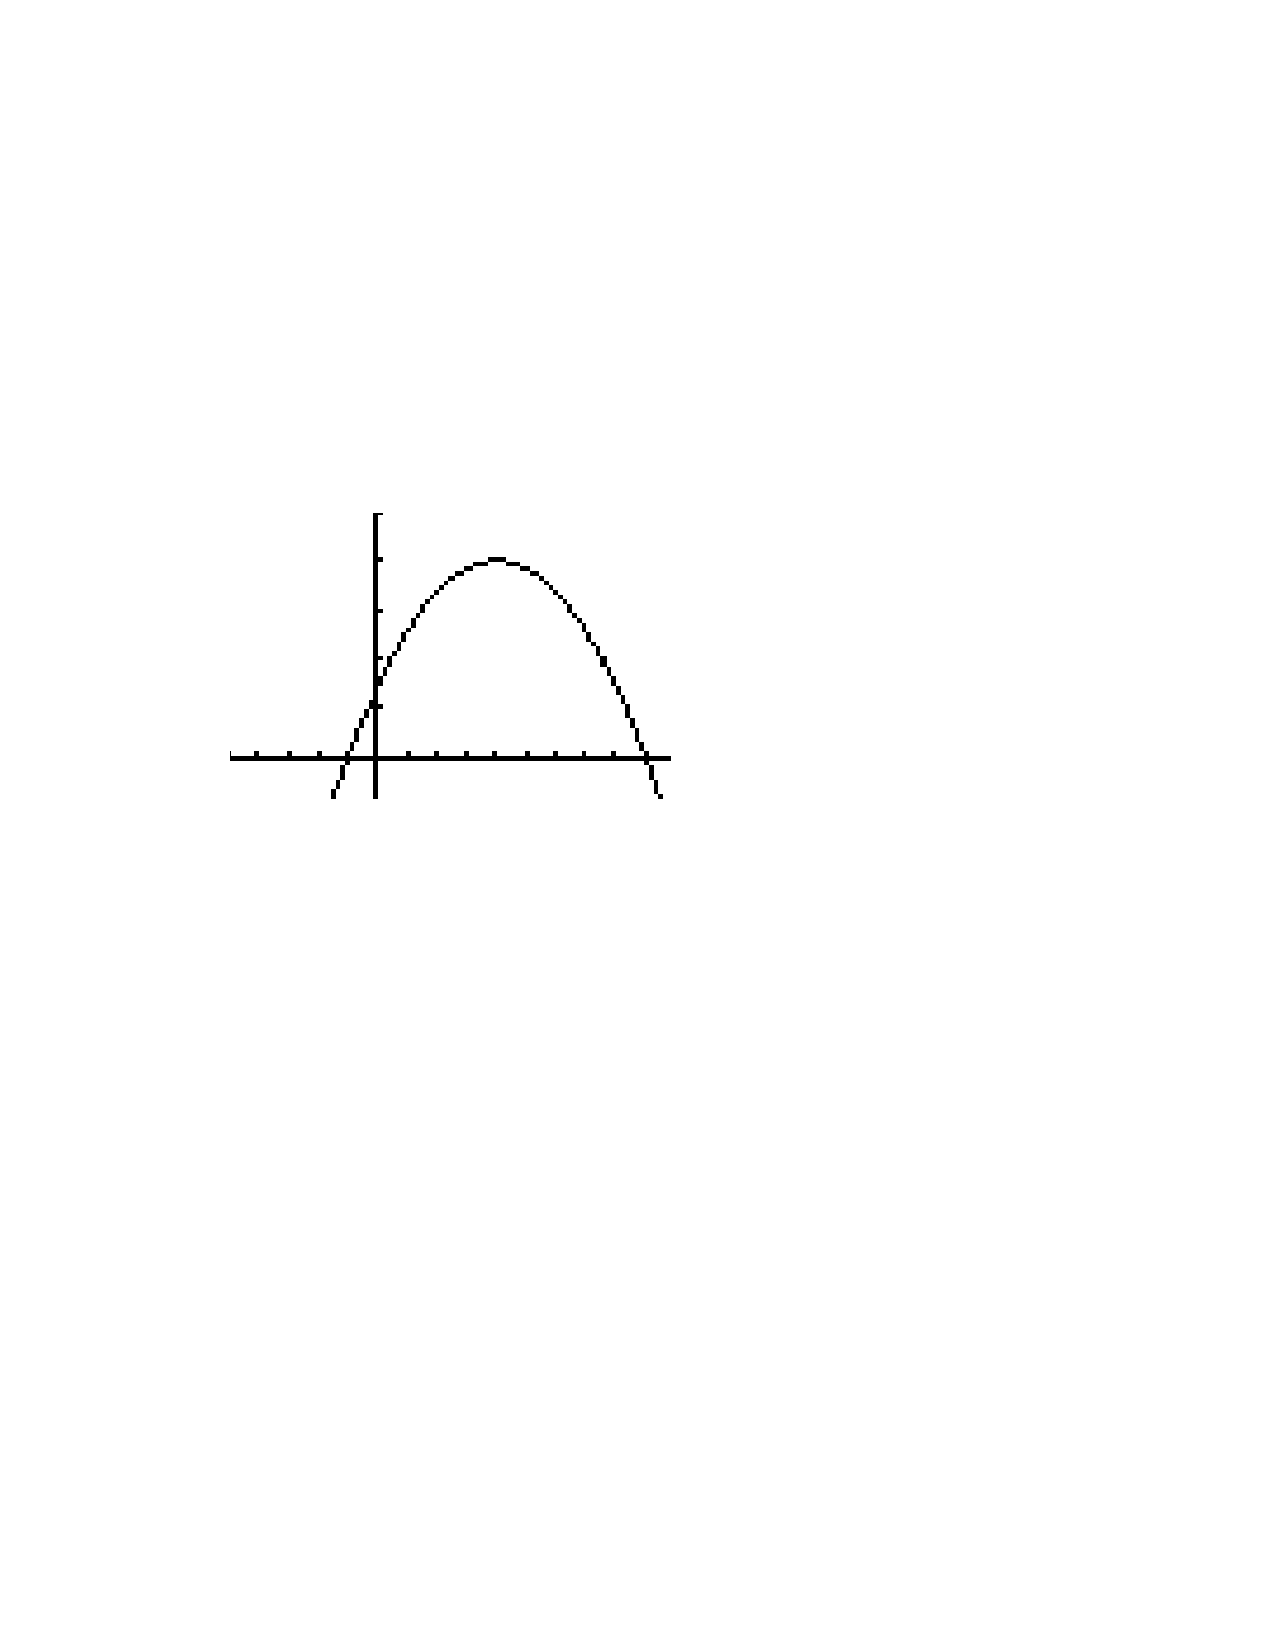
\includegraphics[trim= 170 350 250 90]{Images/Figure1.pdf}
    \end{image}
  \end{quote}
		\begin{freeResponse}
		The error occurs when the student plugs in values for $x$ and $y$ \dfn{before} differentiating the equation $x^2 + y^2 = z^2$ with respect to time.  The distances $x$ and $y$ are clearly changing with respect to time, and so they cannot be treated as constants when we are differentiating.
		
		Differentiating $x^2 + y^2 = z^2$ with respect to $t$ yields:
		$$ 2x \dd[x]{t} + 2y \dd[y]{t} = 2z \dd[z]{t}$$
		
		Canceling the 2's and plugging in the known quantities yields:
		$$ z \dd[z]{t} = (15)(30) + (10)(15) = 450 + 150 = 600 $$
		
		In the above work, the student did correctly compute that $z^2 = 325$ at this fixed instant in time.  So $z = 5\sqrt{13}$, and we can solve for $\dd[z]{t}$ to obtain
		$$ \dd[z]{t} = \frac{600}{5 \sqrt{13}} = \frac{120}{\sqrt{13}} \, mph $$
		\end{freeResponse}	

\end{problem}
\end{document} 
